\chapter{Problem Background}
\label{ch:problem_background}
Jointly the thesis I was willing to develop a neural net model for automatic spine vertebrae segmentation of computer tomography scans (images). CT is a preferred image modality to examine the bone part of a spine due to high bone-to-soft-tissue contrast. As I learned, before proceeding with analysing the bones themselves we need to precisely reconstruct and label our data. Owing to \href{https://biomedia.doc.ic.ac.uk/}{\color{blue}"BioMediaA"} laboratory I was capable to use already collected and labeled dataset. Within this chapter I will reflect the most common core details of the process of segmenting vertebrae CT scans.            

\section{Terminology}
In this section I will introduce terms frequently used in this work: "FCN" - fully connected neural network, "CNN" - convolutional neural network, "detection model" - neural network which stands for set of vertebra apart background, "identification model" - identifies which vertebrate belongs which segmented pixel, "Dice score" - Dice similarity coefficient to quantify the goodness of identification model predictions, "ID rate" - measurement of correctness of detection model predictions. On top of it, based on description of dataset by \href{https://biomedia.doc.ic.ac.uk/}{\color{blue}"BioMediaA"}, the mapping of a class-label-to-vertebra-label is fixed, inherently implying labelling the vertebra.    

\section{Vertebral Segmentation}
Commonly, for vertebral segmentation it was utilized techniques, which naturally comprised aligning a shape-prior to the spine and deforming it such that it fits the given spine. For that it was used geometrical models,  statistical shape models and active contours. But with advent of neural networks and rising of computational power we started developing more complex nets architectures and tune more hyper parameters of them rather than focus on the images and developing a new shape-prior algorithm or others. Thus, neural networks can find such patterns and shapes on the images which frequently scientists can not manage with. Yes, we still need to control the neural net as well as interpret the output, but as for now almost all creative work can be handled by the various net architectures.

As an evidence I can consider Suzani's work \cite{Suzani2015} who proposed to use a multi-layer perceptron to detect the vertebral bodies and employ deformable registration for segmentation. 

Korez \cite{Korez2016} at his work "Model-based segmentation of vertebral bodies from MR images with 3d CNNs" had achieved high accuracy predicting probability maps, which are then used to guide the boundaries of a deformable vertebral model making use of a 3D convolutional neural networks (CNN). 

Moving forward more and more with data-driven decisions, Sekuboyina \cite{Sekuboyina2018} had established a patch-based binary segmentation of the spine using a U-Net, followed by denoising the spine mask using a low-resolution heat map.

At 2018, Janssens \cite{Janssens2018} had successfully performed multi-class segmentation of lumbar vertebrae with two successive CNNs. In the same time at 2018 as well, Lessmann \cite{Lessmann2019} had firstly introduced a two-staged iterative approach, wherein the first stage involves identifying and segmenting one vertebrae after another at a lower resolution, followed a second CNN for refining the lower-resolution masks. Enhancing his approach, at \cite{Lessmann2019} he proposed a single stage FCN which iteratively regresses the vertebrae’s anatomical label and
segments it. Once the entire scan is segmented, the vertebral labels adjusted using a maximum likelihood
technique. 

Eventually, instead of Lessmann's 1-stage and 2-stage iterative solutions and Sekuboyina's patch-wise U-net, at 2020 Payer \cite{Payer2020} had released a coarse-to-fine approach involving three stages, spine localisation, vertebra labelling, and vertebrae segmentation, all three utilising purposefully designed FCNs.

\section{Vertebral Labeling}
\section{Dataset}
\section{Metrics}


\section{Data description}
%TODO change
The data set consists of spine-focused CT scans of 125 patients with varying types of pathologies. 

In the case of the detection model the dense labelling contains two values: 0 representing background and 1 representing vertebrae. 

The identification model’s dense labelling contains values from 0 to 26. Whilst 0 representing background, 1 representing C1 vertebrae up to 26 representing S2 vertebrae.

\begin{figure}[h]
    \centering 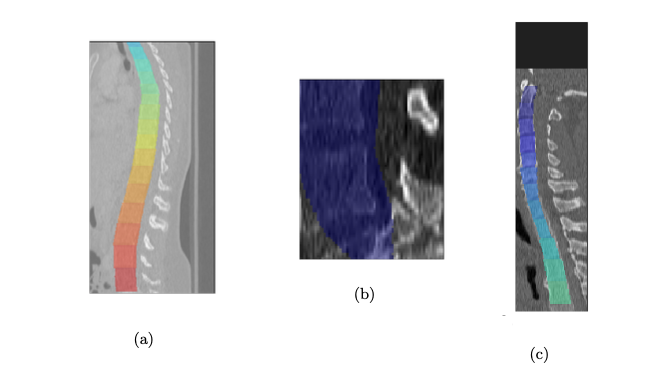
\includegraphics[width=9cm]{images/labeled_data.png}
    \caption {(a) shows a dense labelling, (b) shows an example of a sample used to train the detection model, (c) shows an example of a sample used to train the identification model. Note: The size of the sample is 8 x 80 x 320, if the original scan is not larger enough to fill those dimensions some padding is added, as can be seen at the top.}
    \label{fig:labeled_data}
\end{figure}
